\section{What a long horizon demands}
\label{sec:row-2}

Each strategy buys room by giving up a different kind of recall, so the choice depends on what a long run must carry forward. This section takes up the agents lane of the map: METR's measure of how long the tasks agents complete have grown, the state a long run must carry, and Vending-Bench, the benchmark task behind the running example.

\subsection{Time horizons measure tasks in human time}
\label{sec:it-8-0a}

\bi
\item \textbf{The curve:} success falls as tasks take skilled people longer.
\item \textbf{The horizon:} the task length at 50\% success, 4 minutes for GPT-4.
\item \textbf{In 2025:} Claude 3.7 Sonnet reached a horizon of 1 hour.
\item \textbf{In 2026:} Claude Opus 4.6 reached 12 hours, near the suite's 16-hour limit.
\ei

Thomas Kwa, Ben West, Joel Becker and 22 colleagues at METR, Measuring AI Ability to Complete Long Tasks, arXiv:2503.14499, March 18, 2025, published at NeurIPS 2025 as Measuring AI Ability to Complete Long Software Tasks, with the blog post of March 19, 2025 (metr.org/blog/2025-03-19-measuring-ai-ability-to-complete-long-tasks). This is the navy work of the map's agents lane that opens the long-horizon section. It measures what agents can do in a unit people understand: the time a task takes a skilled person. Its 170 tasks run from software actions of a few seconds (SWAA, 66 tasks) through HCAST (97 tasks, from 1 minute to about 30 hours) to RE-Bench's research engineering tasks of 8 hours (7 tasks). Professionals with about five years of experience made more than 800 baseline attempts, 2,529 hours in all, and a task's time is the geometric mean of the successful attempts.

For each model, METR fits a logistic curve of success against the logarithm of a task's human time. The 50\% time horizon is where the curve crosses one half. The 80\% horizon is where it crosses 80 percent, and it is about five times shorter: in the paper, Claude 3.7 Sonnet's horizons were 59 minutes at 50\% and 15 minutes at 80\%. A horizon describes these tasks, mostly well-specified software tasks that a program can score, and says nothing about how long an agent runs.

The figure draws METR's current numbers, Time Horizon 1.1 of January 2026, with 228 tasks and the fit METR corrected on March 3, 2026, as served on November 5, 2026: GPT-4 at 4 minutes, Claude 3.7 Sonnet at 1 hour (60 minutes) and Claude Opus 4.6 at 12 hours (a 95\% interval of about 5 to 61 hours). Each curve is METR's two-parameter logistic, fixed by the model's published 50\% and 80\% horizons. METR writes that the suite ``can't reliably measure time horizons above 16 hours'' (Frontier Risk Report, May 19, 2026), because too few of its tasks are that long, and the grey band marks where the measure runs out.

Every curve is METR's fit on its Time Horizon 1.1 suite, drawn from the model's published 50\% and 80\% horizons, and nothing is illustrative. The three models are three of METR's frontier models, chosen two years apart. The grey band starts at the 16 hours METR names as the suite's limit.

\begin{figure}[htbp]
\centering
\includegraphics[width=\linewidth]{context/metr-curve-4.png}
\caption{Time horizons measure tasks in human time. The figure as it stands after the build's last click.}
\label{fig:metr-curve-4}
\end{figure}

\paragraph{The figure, stage by stage.}
\be
\item The curve: GPT-4's fitted success rate on METR's tasks against the time each task takes a skilled person, on a log scale from 1 second to 32 hours. Success is near 100\% on tasks of seconds and falls toward zero on tasks of hours.
\item The horizon: the dashed line at 50\%, and GPT-4's 50\% time horizon, ringed at 4 min, where its curve crosses one half. That crossing is the definition.
\item 2025: Claude 3.7 Sonnet's curve lies to the right, and it crosses 50\% at 1 h.
\item 2026: Claude Opus 4.6's curve crosses 50\% at 12 h. The grey band past 16 h marks where METR's suite has too few tasks to measure a horizon reliably, and the caption says so.
\ee

\begin{takeaway}A model's time horizon is the human time of the tasks it completes half the time.\end{takeaway}

\subsection{Time horizons grew from seconds to hours}
\label{sec:it-8-0b}

\bi
\item \textbf{The 2025 paper:} horizons doubled about every seven months to 2025.
\item \textbf{The frontier:} Opus 4.6 reached 12 hours, and Opus 5.5 has no METR horizon.
\item \textbf{Since 2023:} on METR's newer suite, the doubling time is about four months.
\item \textbf{The runs:} METR budgets millions of tokens a task and manages the context.
\ei

The blog post's graph is the paper's Figure 1: eleven frontier models from GPT-2 (2019) to Claude 3.7 Sonnet (February 2025), whose 50\% horizons rise from about 2 seconds to 59 minutes. A least-squares line through their logarithms doubles every 212 days, about seven months (95\% interval 171 to 249 days), with R² 0.98. The NeurIPS version adds o3 and reports 207 days. METR printed no table of that figure, so we recomputed it from METR's runs file at commit 2cd6540, which reproduces every horizon the paper prints.

METR has since moved to a larger suite, Time Horizon 1.1 (228 tasks, January 2026), and it stopped updating its dashboard on September 8, 2026. METR says the two suites are not directly comparable, so the figure draws the newer suite throughout, with GPT-2 to GPT-3.5 carried over from the old one as METR's own chart does. On the newer suite, the frontier models since 2023 double about every 129 days, about four months (95\% interval 104 to 158 days), the fit the figure draws. In 2026, Claude Opus 4.6 reached 12 hours (February), Gemini 3.1 Pro 6.4 hours and GPT-5.4 5.7 hours. Claude Mythos Preview (early) measured 17 hours, above the 16 hours the suite can measure, and GPT-5.6 Sol about 11 hours, which METR calls not a robust measurement. For Claude Opus 5.5, METR's report of September 22, 2026 gives no time horizon: it used five other tasks.

The link to context is the run. METR gives its agents budgets of millions of tokens per task: 2 million for its basic scaffold in 2025, 8 to 16 million for the scaffolds of the o-series models, and 16 to 64 million in 2026. Its scaffold ``manages the model's context by organizing its inputs and ensuring they do not exceed the model's maximum context window'' (METR's o3 report, 2025). A task of hours is a run of many calls whose history outgrows one window, the problem of the rest of this section.

Every point is a horizon METR published for a model it marks as the frontier when released, with METR's 95\% interval. The fit is ours, computed as METR describes, and it reproduces METR's 128.7 days. Models that were not the frontier when released, such as Claude Opus 4.1 and Gemini 3.1 Pro, are left out, and the notes give their horizons where they matter.

\begin{figure}[htbp]
\centering
\includegraphics[width=\linewidth]{context/metr-trend-5.png}
\caption{Time horizons grew from seconds to hours. The figure as it stands after the build's last click.}
\label{fig:metr-trend-5}
\end{figure}

\paragraph{The figure, stage by stage.}
\be
\item Seconds: each point is a frontier model's 50\% time horizon on METR's tasks, with its 95\% interval, at its release date, on a log scale from 1 second to 48 hours. GPT-2 (2019), GPT-3 and GPT-3.5 (2022) complete tasks of a few seconds.
\item Minutes: the frontier models of 2023 and 2024, from GPT-4 at 4 minutes to o1 at 39 minutes.
\item Hours: the frontier models of 2025, from Claude 3.7 Sonnet at 1 hour to GPT-5.2 at about 6 hours.
\item 2026: Claude Opus 4.6 at 12 hours, and Claude Mythos Preview, hollow at 17 hours in the grey band past 16 hours, where METR says its suite has too few tasks to measure.
\item The trend: the dashed line fits the frontier models since 2023 that stay under 16 hours, doubling every 129 days, about four months.
\ee

\begin{takeaway}Tasks of many hours make runs that must manage their context.\end{takeaway}

\subsection{Long runs accumulate state to preserve}
\label{sec:it-8-1}

\bi
\item \textbf{Goals and plans} set what the run is for and how it intends to get there.
\item \textbf{Progress and open commitments} record work done and promises pending.
\item \textbf{Grounded evidence} keeps the observations a later decision will rest on.
\item \textbf{Replanning triggers} mark when new observations should change the plan.
\ei

The strategies showed what each one gives up. A long run shows what it must not lose. A long run accumulates state that later calls need: the goals and the plan, the progress so far and the commitments still open, the evidence that later decisions rest on, and the conditions that should trigger a new plan. The vending run the figures have followed is a Vending-Bench task, and its paid order is an open commitment.

The course combines ideas from two sources. Justin Young's Effective harnesses for long-running agents (Anthropic, November 26, 2025) discusses progress records and verification. That article is engineering guidance and measures nothing. LLM-Planner (Chan Hee Song, Jiaman Wu, Clayton Washington, Brian M. Sadler, Wei-Lun Chao and Yu Su, LLM-Planner: Few-Shot Grounded Planning for Embodied Agents with Large Language Models, ICCV 2023) addresses grounded replanning. The slide \hyperref[sec:it-7-5]{``Real harnesses compact, delegate and retry.''} gave QwenGyre's scale: runs of hours, hundreds of interactions and nearly 1M tokens. The previous slides showed that the tasks agents complete keep getting longer, so the state a run must carry grows with them. The next sections test whether the pending commitment of Day 1 survives compaction.

The record, the price and the days in the figure are the course's illustrative teaching case.

\begin{figure}[htbp]
\centering
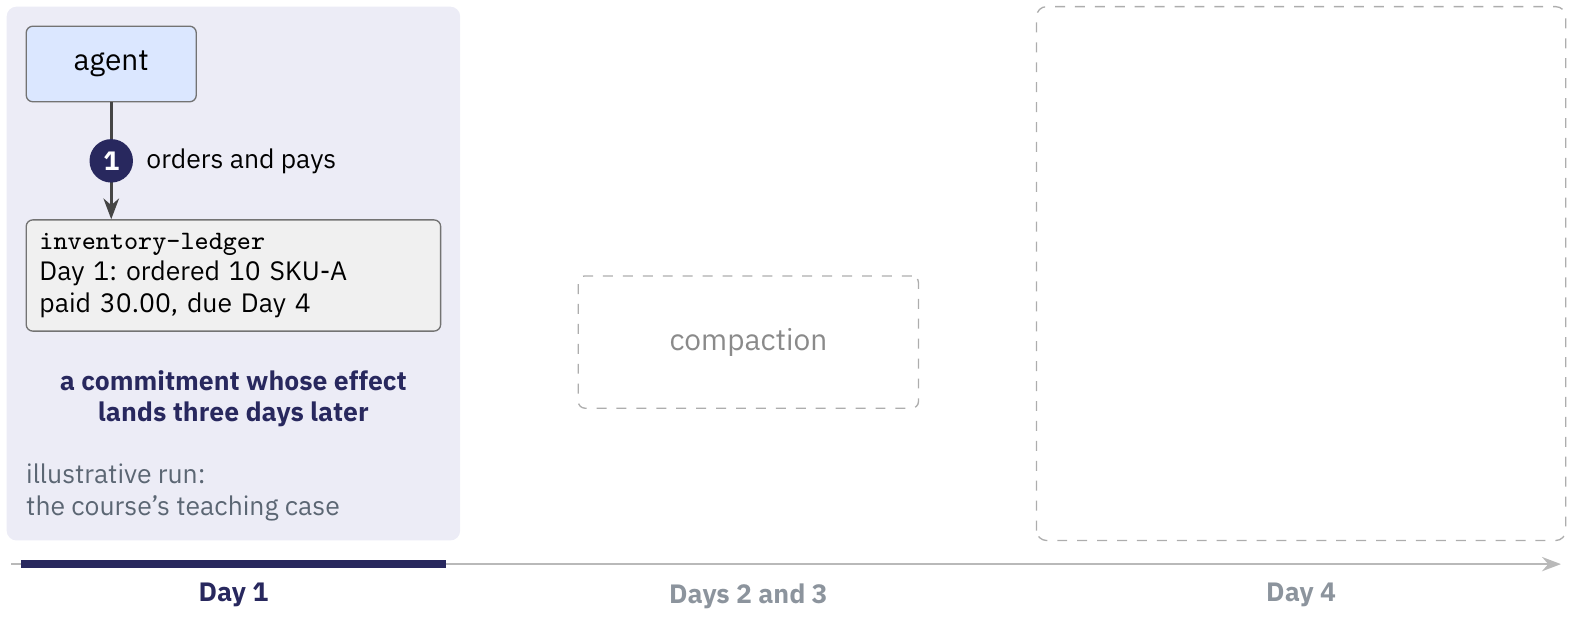
\includegraphics[width=\linewidth]{context/dropped-order-1.png}
\caption{Long runs accumulate state to preserve. The figure as it stands after the build's last click.}
\label{fig:dropped-order-1}
\end{figure}

\paragraph{The figure, stage by stage.}
\be
\item Day 1: the agent ``orders and pays'', and the inventory-ledger records ``Day 1: ordered 10 SKU-A'' and ``paid 30.00, due Day 4'', which the navy caption calls ``a commitment whose effect lands three days later''. The grey note reads ``illustrative run: the course's teaching case'', and dashed ghosts hold the places of compaction and Day 4.
\ee

\begin{takeaway}A long run must carry its open commitments forward to act well.\end{takeaway}

\subsection{Vending-Bench stresses long-term coherence}
\label{sec:it-8-2}

\bi
\item \textbf{The task:} an agent runs a vending business (Andon Labs, preprint, 2025).
\item \textbf{The horizon:} many simulated days, with delayed deliveries and a daily fee.
\item \textbf{The reported failure:} some long runs misread deliveries, full window or not.
\item \textbf{Why it fits:} the run's state outgrows one context and must be carried forward.
\ei

Axel Backlund and Lukas Petersson (Andon Labs), Vending-Bench: A Benchmark for Long-Term Coherence of Autonomous Agents, arXiv:2502.15840, February 20, 2025, a preprint. This is the navy work of the map's agents lane, the task Part II studies in depth, and the vending run the figures have followed is set in it. The agent runs a vending-machine business over simulated calendar time: it checks inventory, orders stock, sets prices and pays a daily fee. Decisions span many simulated days, orders arrive after a delivery delay, and the fee recurs. Over long runs, agents can lose long-term coherence: they misread stock and deliveries, and in some runs they wind the business down early. The run's state outgrows one context, so the agent must preserve information between calls.

Andon Labs released Vending-Bench 2 on November 18, 2025 (andonlabs.com/evals/vending-bench-2, a benchmark page with a leaderboard) and now marks the original as deprecated. Vending-Bench 2 runs a simulated year and adds adversarial suppliers, deliveries that arrive later than promised and suppliers that go out of business. Part II studies the task as the 2025 paper defines it.

Jimenez et al., SWE-bench: Can Language Models Resolve Real-World GitHub Issues?, ICLR 2024 (arXiv:2310.06770v2, April 2024), shows that real GitHub issues are hard for language models: resolving one often needs coordinated edits across several functions and files. With BM25 retrieval and one generated patch per issue, the best of the models in that version, Claude 2, resolved 1.96\% of 2,294 issues, and 4.8\% when given the files the reference patch edited. The paper evaluates no agents, and these rates hold only for the 2023 models and that setup. We keep the simulated calendar duration distinct from the agent's wall-clock runtime and from the depth of its plan. The exact Vending-Bench figures stay in the source paper. Our delayed-delivery case illustrates the paper's type of coherence failure.

The run in the figure is the course's teaching case. In the paper, the agent sees the last 30,000 tokens of its history in most experiments, together with a scratchpad, a key-value store and a vector database, and no summary step. Products arrive a few days after an order, and a daily fee recurs. The authors find no clear correlation between the failures and the point at which the model's context window fills, and their examples include ordering new stock instead of restocking from storage, believing that orders had arrived before they had, and announcing the closure of the business. The compaction step in our figure therefore illustrates the class of failure the paper reports, and we attribute none of the paper's failures to compaction.

\begin{figure}[htbp]
\centering
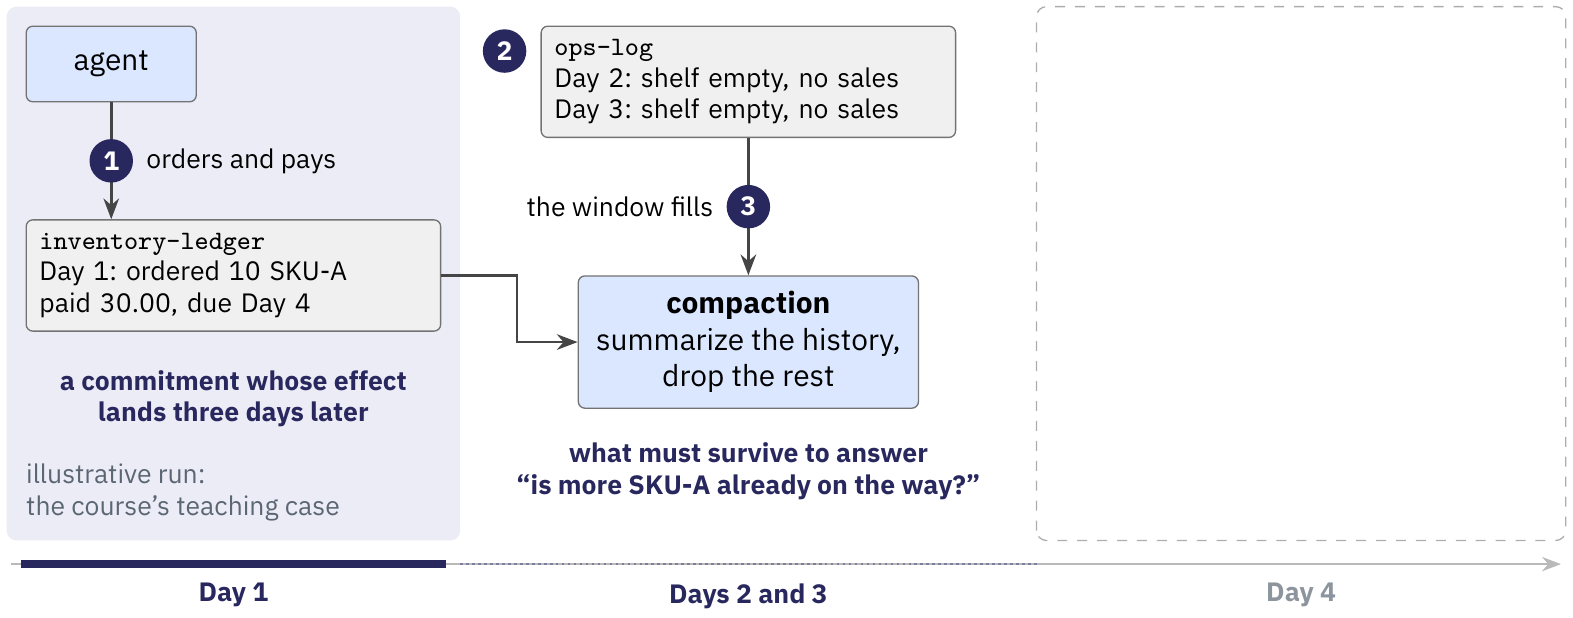
\includegraphics[width=\linewidth]{context/dropped-order-2.png}
\caption{Vending-Bench stresses long-term coherence. The figure as it stands after the build's last click.}
\label{fig:dropped-order-2}
\end{figure}

\paragraph{The figure, stage by stage.}
\be
\item Day 1: the agent ``orders and pays'', and the inventory-ledger records ``Day 1: ordered 10 SKU-A'' and ``paid 30.00, due Day 4'', which the navy caption calls ``a commitment whose effect lands three days later''. The grey note reads ``illustrative run: the course's teaching case'', and dashed ghosts hold the places of compaction and Day 4.
\item The ops-log for Days 2 and 3 records ``Day 2: shelf empty, no sales'' and ``Day 3: shelf empty, no sales'', and when ``the window fills'', compaction reads the ledger and the log to ``summarize the history, drop the rest''. The navy question asks ``what must survive to answer ``is more SKU-A already on the way?''''.
\ee

\begin{takeaway}A long run forces a choice about what to carry forward.\end{takeaway}

\subsection*{Key points}
\bi
\item A model's time horizon is the human time of the tasks it completes half the time.
\item Tasks of many hours make runs that must manage their context.
\item A long run must carry its open commitments forward to act well.
\item A long run forces a choice about what to carry forward.
\ei
